% Options for packages loaded elsewhere
\PassOptionsToPackage{unicode}{hyperref}
\PassOptionsToPackage{hyphens}{url}
\documentclass[
  11pt,
]{article}
\usepackage{xcolor}
\usepackage[margin=1.0in]{geometry}
\usepackage{amsmath,amssymb}
\setcounter{secnumdepth}{-\maxdimen} % remove section numbering
\usepackage{iftex}
\ifPDFTeX
  \usepackage[T1]{fontenc}
  \usepackage[utf8]{inputenc}
  \usepackage{textcomp} % provide euro and other symbols
\else % if luatex or xetex
  \usepackage{unicode-math} % this also loads fontspec
  \defaultfontfeatures{Scale=MatchLowercase}
  \defaultfontfeatures[\rmfamily]{Ligatures=TeX,Scale=1}
\fi
\usepackage{lmodern}
\ifPDFTeX\else
  % xetex/luatex font selection
\fi
% Use upquote if available, for straight quotes in verbatim environments
\IfFileExists{upquote.sty}{\usepackage{upquote}}{}
\IfFileExists{microtype.sty}{% use microtype if available
  \usepackage[]{microtype}
  \UseMicrotypeSet[protrusion]{basicmath} % disable protrusion for tt fonts
}{}
\makeatletter
\@ifundefined{KOMAClassName}{% if non-KOMA class
  \IfFileExists{parskip.sty}{%
    \usepackage{parskip}
  }{% else
    \setlength{\parindent}{0pt}
    \setlength{\parskip}{6pt plus 2pt minus 1pt}}
}{% if KOMA class
  \KOMAoptions{parskip=half}}
\makeatother
\usepackage{graphicx}
\makeatletter
\newsavebox\pandoc@box
\newcommand*\pandocbounded[1]{% scales image to fit in text height/width
  \sbox\pandoc@box{#1}%
  \Gscale@div\@tempa{\textheight}{\dimexpr\ht\pandoc@box+\dp\pandoc@box\relax}%
  \Gscale@div\@tempb{\linewidth}{\wd\pandoc@box}%
  \ifdim\@tempb\p@<\@tempa\p@\let\@tempa\@tempb\fi% select the smaller of both
  \ifdim\@tempa\p@<\p@\scalebox{\@tempa}{\usebox\pandoc@box}%
  \else\usebox{\pandoc@box}%
  \fi%
}
% Set default figure placement to htbp
\def\fps@figure{htbp}
\makeatother
% definitions for citeproc citations
\NewDocumentCommand\citeproctext{}{}
\NewDocumentCommand\citeproc{mm}{%
  \begingroup\def\citeproctext{#2}\cite{#1}\endgroup}
\makeatletter
 % allow citations to break across lines
 \let\@cite@ofmt\@firstofone
 % avoid brackets around text for \cite:
 \def\@biblabel#1{}
 \def\@cite#1#2{{#1\if@tempswa , #2\fi}}
\makeatother
\newlength{\cslhangindent}
\setlength{\cslhangindent}{1.5em}
\newlength{\csllabelwidth}
\setlength{\csllabelwidth}{3em}
\newenvironment{CSLReferences}[2] % #1 hanging-indent, #2 entry-spacing
 {\begin{list}{}{%
  \setlength{\itemindent}{0pt}
  \setlength{\leftmargin}{0pt}
  \setlength{\parsep}{0pt}
  % turn on hanging indent if param 1 is 1
  \ifodd #1
   \setlength{\leftmargin}{\cslhangindent}
   \setlength{\itemindent}{-1\cslhangindent}
  \fi
  % set entry spacing
  \setlength{\itemsep}{#2\baselineskip}}}
 {\end{list}}
\usepackage{calc}
\newcommand{\CSLBlock}[1]{\hfill\break\parbox[t]{\linewidth}{\strut\ignorespaces#1\strut}}
\newcommand{\CSLLeftMargin}[1]{\parbox[t]{\csllabelwidth}{\strut#1\strut}}
\newcommand{\CSLRightInline}[1]{\parbox[t]{\linewidth - \csllabelwidth}{\strut#1\strut}}
\newcommand{\CSLIndent}[1]{\hspace{\cslhangindent}#1}
\setlength{\emergencystretch}{3em} % prevent overfull lines
\providecommand{\tightlist}{%
  \setlength{\itemsep}{0pt}\setlength{\parskip}{0pt}}
\usepackage{helvet} % Helvetica font
\renewcommand*\familydefault{\sfdefault} % Use the sans serif version of the font
\usepackage[T1]{fontenc}

\usepackage[none]{hyphenat}

\usepackage{setspace}
\doublespacing
\setlength{\parskip}{1em}

\usepackage{lineno}

\usepackage{pdfpages}
\usepackage{bookmark}
\IfFileExists{xurl.sty}{\usepackage{xurl}}{} % add URL line breaks if available
\urlstyle{same}
\hypersetup{
  pdftitle={Evidence for a Change to Aerosol Fractions: In a Gobi Town},
  hidelinks,
  pdfcreator={LaTeX via pandoc}}

\title{\textbf{Evidence for a Change to Aerosol Fractions: In a Gobi
Town}}
\author{}
\date{\vspace{-2.5em}}

\begin{document}
\maketitle

\vspace{35mm}

Running title: INSERT RUNNING TITLE HERE

\vspace{35mm}

Munkhtsetseg, Shimizu. A, Matsuki. A, Batdorj. D, Matsui. H

\vspace{40mm}

To whom correspondence should be addressed:

\newpage
\linenumbers

\subsection{Abstract (150 words)}\label{abstract-150-words}

Driven by mining industrial progress, household coal combustion has
increased greatly in Mongolia since the 2000s. Demographic evidence has
revealed an ongoing reduction in rural-nomadic lifestyle and a rise of
the population at urban areas, which may gradually extend a household
winter heating as a major source of fine particulate matter (PM2.5).
Together ff with observations that lifespan in various animal species is
flexible and can be increased by genetic or pharmaceutical intervention,
these results have led to suggestions that longevity may not be subject
to strict, species-specific genetic constraints. Here, by analysing
global demographic data, we show that improvements in survival with age
tend to decline after age 100, and that the age at death of the world's
oldest person has not increased since the 1990s. Our results strongly
suggest that the maximum lifespan of humans is fixed and subject to
natural constraints. Storyline:

\begin{enumerate}
\def\labelenumi{\arabic{enumi}.}
\tightlist
\item
  A new pattern is emerged
\item
  Air quality in urban sites is episodically dictated by dust events in
  spring or late autumn, yet seasonally governed by anthropogenic
  emissions in winter. {[}Air quality is governed by natural dust
  emission, and anthropogenic emissions{]}
\item
  With recent growing interest in urban life style, and combustion of
  coal/oyutolgoi for heating winter conditions results a highly increase
  in not only capital city but also towns
\item
  In a result, spring coarse dust, plus winter fine pollutants
\item
  spring coarse dust is immediately transported and deposited in the
  source area, whereas winter fine pollutants is permanently stayed in
  the source area due to stagnant atmosphere govern over entire
  country., perhaps floating in the near surface, deposits in the
  surface{]}
\item
  Alarms, the Mongolian dust in the spring, optical properties might be
  shifted; this gives \ldots{} Gobi dust and sand storms has become
  tuiren, from the shoroon shuurga. which clearly requires the
  attention.
\item
  r ratio shows \ldots{} emission source; dust might carry anthropogenic
  fine particulates as well. Spatio-temporal distinct patterns in
  variations of \(PM_{10}\) and \(PM_{2.5}\) relative to the recent
  drivings of emission sources in Mongolia \newpage
\end{enumerate}

\subsection{Introduction}\label{introduction}

\begin{itemize}
\item
  Advanced the knowledge of global dust, has reached to recognize the
  sources,.
\item
  Classification dust brown color, seasonal characteristics, with coarse
  fractions.
\item
  This knowledge further efficient to climate system when elaborating
  dust-aerosol effects.
\item
  But, a large uncertainties in the global dust model has existed so for
  climate models which clearly limits our understanding the climate
  system and shape the facing global issues of global warming.
\item
  This is mainly caused by the lack of parameterization and recognition
  of iterative changes controlled by the natural forces and
  anthropogenic drivings.
\item
  Mongolian dust brown color, seasonal characteristics, with coarse
  fractions.
\item
  Mongolian dust has an attention of the its mass fraction in global
  dust, yet unlikely elaborated in the climate models due to its
  majority of coarse fraction for its a small contribution to the
  climate system through its radiative feedback.
\item
  But, such recognized characterization might get no longer valid due to
  recent change in the driving of the emissions of air particulate
  matters. A large high concentrations of PM2.5 in the capital city of
  Mongolia has been observed as a result of the heavy consumptions of
  coal as a winter heating has rapidly spread as a mining industry taken
  off since 2000. Winter weather stagnant conditions governed by the
  Siberian magnifies the concentrations of the particulate matter
  emissions by trapping the polluted air below the boundary layer, so
  that results in a very large high concentrations of PM2.5, locally.
  Even recognized as one of the highly polluted capital cities in the
  world.
\item
  Therefore, It is important to examine the emerging changes and
  shifting patterns of air particulate matters in Mongolia. More
  importantly, it is essential to reveal the significant changes in the
  the altered fraction particularly, in the dust seasons considering its
  high potential of intriuging in the free atmosphere to transported in
  the long-distance, so carrying capacity of the role to shift the
  global climate system, and its side impacts on downwind regions.
\item
  Study goal - We hypothesize \ldots{} - Our study will benefit not only
  to the global dust research but also climate, and further to the
  country itself for urban planning, and coal combustion.
\end{itemize}

\subsubsection{Research Qs}\label{research-qs}

Therefore, we aimed to demonstrate the distinct temporal and spatial
variations of PM2.5 and PM10 across urban and rural Mongolia using
extensive data from 2008 to 2020.

On spring, the dust storm from the Gobi Desert contribute significantly
to increased aerosols in the atmosphere and ambient air pollution,
leading to sporadic peaks in PM10 concentrations reaching as high as
64-234 \(\mu g m^{-3}\) per day or exceeding 6000 \(\mu g m^{-3}\) per
hour (Jugder). concentrations of particulate matter is ephederemal, yet
vary depending on whether the pollution cause is natural or industrial,
local or transported, seasonal or non-seasonal, makes complex and
challenging. 1. Do concentrations of particulate matters differ in
between urban and rural sites, and even within Gobi sites? 2. Do
distinct temporal variations has existed among the sites? 3. Do PM2.5
particulates has contributed to the PM10 annual variations?

\begin{itemize}
\tightlist
\item
  If yes, how much, and when and where?
\item
  What is the sd, mean, and median

  \begin{itemize}
  \tightlist
  \item
    box plot
  \item
    violin
  \item
    scatter points, epidemic, sporadic
  \end{itemize}
\item
  Daily variations to examine it related to the heating

  \begin{itemize}
  \tightlist
  \item
    2 peaks: smaller and bigger
  \item
    compare the t-duration exceeds 50mug/m3/hour
  \end{itemize}
\end{itemize}

\begin{enumerate}
\def\labelenumi{\arabic{enumi}.}
\setcounter{enumi}{3}
\tightlist
\item
  Does it has distinct patterns among the sites regarding to the
  drivings
\end{enumerate}

\begin{itemize}
\tightlist
\item
  How PMs varies with the wind speed and visibility
\item
  Do they differently explained with variables and changes in drivings
  (with PCA analysis)
\end{itemize}

\begin{enumerate}
\def\labelenumi{\arabic{enumi}.}
\setcounter{enumi}{4}
\tightlist
\item
  Is there any significant changes in time-series of PMs at 4 seasons
\item
  Is there any significant changes in ratio in the spring in respect to
  winter?
\end{enumerate}

The present study will contribute significantly to the understanding of
air particulate matter patterns in Mongolia and providing comprehensive
data insights for policymakers and public health sectors. Our findings
is useful not only for addressing national health impacts but also
beneficial for understanding air particulate matter as ambient air
pollution, and tackling atmospheric aerosol effects in the climate
system, and revealing their transboundary effects to the downwind
regions in South-east Asia.

\subsection{Results}\label{results}

\subsubsection{The spatio-temporal variations of the PMs at the study
sites}\label{the-spatio-temporal-variations-of-the-pms-at-the-study-sites}

To evaluate the spatial variations in particulate matter (PM)
concentrations, we displayed hourly observed values of PM10 and PM2.5
for all study sites (figure\_3). The mean p-values indicate that PM
concentrations differ significantly at a 99\% confidence level across
all sites (figure\_3), with the exception of a 95\% confidence level
between DZ and UB for PM10 (figure\_3a), highlighting substantial
concentration disparities among sites. While quantitative differences in
PM concentration values exist across all sites, two key patterns emerge
when examining median deviations from mean values and irregular
observation fluctuations. For instance, PM10 demonstrates more erratic
behavior than PM2.5 at each location, particularly evident at ZU and SS
sites. Furthermore, the mean values calculated from hourly measurements
surpass the median concentrations for both PM10 and PM2.5 across all
sites, with notable prominence at UB and DZ locations. Consequently,
significant spatial differences in PM concentrations exist among all
sites, regardless of urban or rural classification. However, the sites
can be categorized into two groups based on their characteristics: UB
(urban) and DZ (rural town, Gobi); and SS (rural, Gobi) and ZU (rural,
Gobi). These findings for DZ appear to support our hypothesis of
emerging new emission patterns related to increased coal consumption
during winter months.

To investigate whether emerging PM patterns are associated with
household winter heating activities, we demonstrated annual variations
in PM10 and PM2.5 concentrations at the sites. Significant annual
variations in PM10 and PM2.5 levels were observed at UB and DZ sites,
with maximum concentrations exceeding 100 \(\mu g/m^3\) during colder
months (January, November, December) and lower levels consistently below
50 \(\mu g/m^3\) during warmer months (May-September). These annual
maximums coincided with the diurnal variations in PM10 and PM2.5
concentrations at sites DZ and UB, where PM concentrations reached their
highest values during nighttime and early morning hours (approximately 8
PM to 4 AM UTC), with median values surpassing 50 \(\mu g/m^3\).
Conversely, both pollutants exhibited reduced concentrations during
daytime hours (8AM to 4PM UTC), likely due to increased atmospheric
dispersion. UB site exhibited similar daily fluctuations with extended
periods (approximately 8 PM to 5 AM UTC) of elevated concentrations.
Additionally, winter PM10 concentrations at both sites were primarily
composed of PM2.5 (figure\_5; mean values for PM10 with the color bar).
The increase in PM10 and PM2.5 aligns with the heating active hours,
suggesting that household coal consumption contributes to elevated PM
levels at both DZ and UB sites. In contrast, ZU and SS sites displayed
significantly lower annual PM10 and PM2.5 levels, with sudden frequent
spikes in spring followed by occasional instances in autumn. These
annual variations were more pronounced in PM10 compared to PM2.5,
highlighting the impact of Gobi dust and sand storms. Similar
occurrences were also noted at the DZ site, suggesting its exposure to
both winter heating emissions and natural spring dust, reflecting its
Gobi-region characteristics. The annual variability in PMs with higher
concentrations during nighttime and colder months, indicating the
influence of localized emission sources and reduced boundary layer
mixing at UB and DZ sites. Additionally, the upward extended ranges
without the bottom bottle of the violin plot, demonstrating greater
variability during colder months. It implies instability in
concentrations potentially reaching high levels above 400 \(\mu g/m^3\)
when Arctic oscillation/Siberian high intensifies with heating, and
dropping below 50 \(\mu g/m^3\) when it weakens or heating demand
decreases. These findings confirm the (DZ) emerging PM pattern is caused
by household activities and influenced by meteorological conditions.
Overall, meteorological factors appear to play a crucial role in
governing PM levels.

\subsubsection{The emission patterns of interrelations among
meteorological variables at the study
sites}\label{the-emission-patterns-of-interrelations-among-meteorological-variables-at-the-study-sites}

add table, add r 1.3, 2 on figure\_6, add supplement figures

To identify the key factors influencing PM emissions, we examined the
relationships between wind speed (WS), visibility (VIS), and particulate
matter (PM10 and PM2.5) concentrations across the study sites
(figure\_6). In UB during winter, elevated PM levels typically coincide
with low wind speeds and reduced visibility (indicated by darker blue
points). Notably, at DZ and ZU locations, high PM10 concentrations were
observed during both low and high wind speed conditions in winter. All
Gobi sites exhibit the greatest variation in PM concentrations during
spring, with extreme outliers primarily associated with increased WS and
reduced visibility below 10000 km. Similar findings were also revealed
through Principal Component Analysis (PCA). The initial two principal
components (Dim 1 and Dim 2) account for 66.52\% of the total variance.
Dim 1 shows a strong association with PM10 and PM2.5, while visibility
demonstrates an inverse correlation, suggesting that reduced visibility
corresponds to higher pollution levels. Wind speed and direction align
positively with Dim 2 (22.16\%), reflecting their impact on emissions.
When comparing PM10 aligns with PM2.5, the 1:1 ratio increases
approximately 1.3 times for UB, 2 times for DZ, XXX for ZU, and XXX for
SS as PM10 concentrations increase. This increase in Gobi sites further
escalated up to 2-5 times in ZU, and XXX times in SS sites, indicating
insufficient PM2.5 particulates in those locations, particularly at the
ZU site. It is worth noting that instances where PM2.5 values exceed
PM10 reflect equipment accuracy, correction errors, and higher
sensitivity rates (ability to record emissions such as smoking near the
sensor area). However, this discrepancy diminishes as PM concentrations
increase, validating that higher observational records of PM2.5 compared
to PM10 do not invalidate our results. Furthermore, clustering of
monitoring sites based on PM concentrations and geographic features
(Figure 7b) reveals distinct patterns. UB (urban, capital city) is
characterized by high PM concentrations (positive Dim 1 scores), while
SS (rural, Gobi, town (site located in the prevailing wind above the
town)) shows low PM levels, clustering tightly along the negative Dim 1
axis. DZ (rural, Gobi, town center) displays considerable variability,
with clusters extending into higher Dim 1 and Dim 2 ranges, reflecting
the complex interplay of emission sources and meteorological factors. ZU
(rural, Gobi, village) overlaps with SS but exhibits greater spread,
indicating moderate pollution levels influenced by seasonal and
localized factors. These findings highlight the complex interplay of
spatial, meteorological, and local factors influencing air particulate
matter concentrations across the studied locations and emphasizing the
need for considering not only regional influences but also site-specific
characteristics.

fig caption: the Principal Component Analysis (PCA) bi-plot (Figure 7a)
highlights the relationships among key variables, including PM10, PM2.5,
wind speed (WS), wind direction (WD), visibility, ratio of PM2.5 to PM10
(r), and numbers of aerosols by optical particle counter (OPC). The
first two principal components (Dim 1 and Dim 2) explain 66.52\% of the
total variance, with Dim 1 (44.36\%) strongly associated with PM10 and
PM2.5. Wind speed and wind direction are positively aligned with Dim 2
(22.16\%), reflecting their influence on pollutant dispersion.

\subsubsection{The recent trends in concentrations of PMS and
fine-coarse fractional changes at the
sites}\label{the-recent-trends-in-concentrations-of-pms-and-fine-coarse-fractional-changes-at-the-sites}

add table, add trend figure: r, add relationship figure: r in spring and
pm2.5 in winter

Figure 8 illustrates the trend analysis of PM10 and PM2.5 concentrations
across study sites from 2009 to 2020. The time series demonstrates
seasonal patterns and trends, with p-values of trend changes,
seasonally: winter (Q1), spring (Q2), and summer-autumn (Q3). At UB,
significant negative trends both in PM10 and PM2.5 concentrations are
observed for winter and spring (Q1 and Q2, p \textless{} 0.001). At DZ,
a significant positive trend in PM10 and PM2.5 concentrations is
observed for winter (Q1, p \textless{} 0.001), indicating increasing
particulate matter levels during this season. At ZU, a significant
negative trend is observed in both PM10 and PM2.5 for winter (Q1, p
\textless{} 0.001), suggesting a consistent reduction in particulate
matter during winter months (may reduced transboundary traffic
associated with covid periods, resulted in declined PM10 concentrations;
or data gaps). At SS, a negative trend is observed in PM2.5 for spring
(Q2, p \textless{} 0.001), reflecting a seasonal decline potentially
linked to reduced wind speed during spring. The significant decreasing
trends in PM concentrations in UB during colder months likely indicate
improvements in emission control measures and a transition to more
efficient heating practices. In contrast, a significant increasing trend
is observed at DZ, particularly during winter (Q1), suggesting rising
emissions potentially associated with urbanized household practices and
other local activities in Mongolia's regional towns.

\subsection{Conclusions}\label{conclusions}

In this study, we investigated the temporal variations of PM2.5 and PM10
concentrations at the 4 sites of rural and urban those located along the
the wind corridor. Air particulate matter concentrations in urban-town
sites of UB and DZ is episodically dictated by dust events in spring or
late autumn, yet seasonally governed by anthropogenic emissions in
winter. Air particulate matter concentrations in rural sites of SS and
ZU is episodically dictated by dust events in spring or late autumn.

Three distinct variations has been detected.

\begin{enumerate}
\def\labelenumi{\arabic{enumi}.}
\tightlist
\item
  It is evident of the new emission patterns in Mongolia.
\item
  Related to the winter emission patterns, fine particulates fraction in
  the spring is increased.
\item
  This alarms\ldots{}
\item
  National level; meteorological impact is large. \ldots{} However,
  reduced\ldots{} On the other hand, it is \ldots{} with the towns. This
  points that air quality will be poor whether it is changed fuel, ..
  unless to change heating system. Therefore, it is not the reason to
  move the capital city. Only solution is to change the heating system,
  do not burn any type of the coal.
\end{enumerate}

\begin{itemize}
\tightlist
\item
  Due to rapid increase in urban, and combustion of coal/oyutolgoi for
  heating winter conditions results a highly increase in not only
  capital city but also towns
\item
  In a result, spring coarse dust, plus winter fine pollutants {[}spring
  coarse dust is immediately transported and deposited in the source
  area, whereas winter fine pollutants is permanently stayed in the
  source area due to stagnant atmosphere govern over entire country.,
  perhaps float- ing in the near surface, deposits in the surface{]}
\item
  Alarms, the Mongolian dust in the spring, optical properties will be
  shifted; this gives \ldots{} Gobi dust and sand storms has become
  tuiren, from the shoroon shuurga. which clearly requires the
  attention.
\end{itemize}

Following problems

\begin{itemize}
\tightlist
\item
  On downwind regions
\item
  On national-level Demonstrating temporal and spatial variations of
\end{itemize}

\newpage

\begin{figure}
\centering
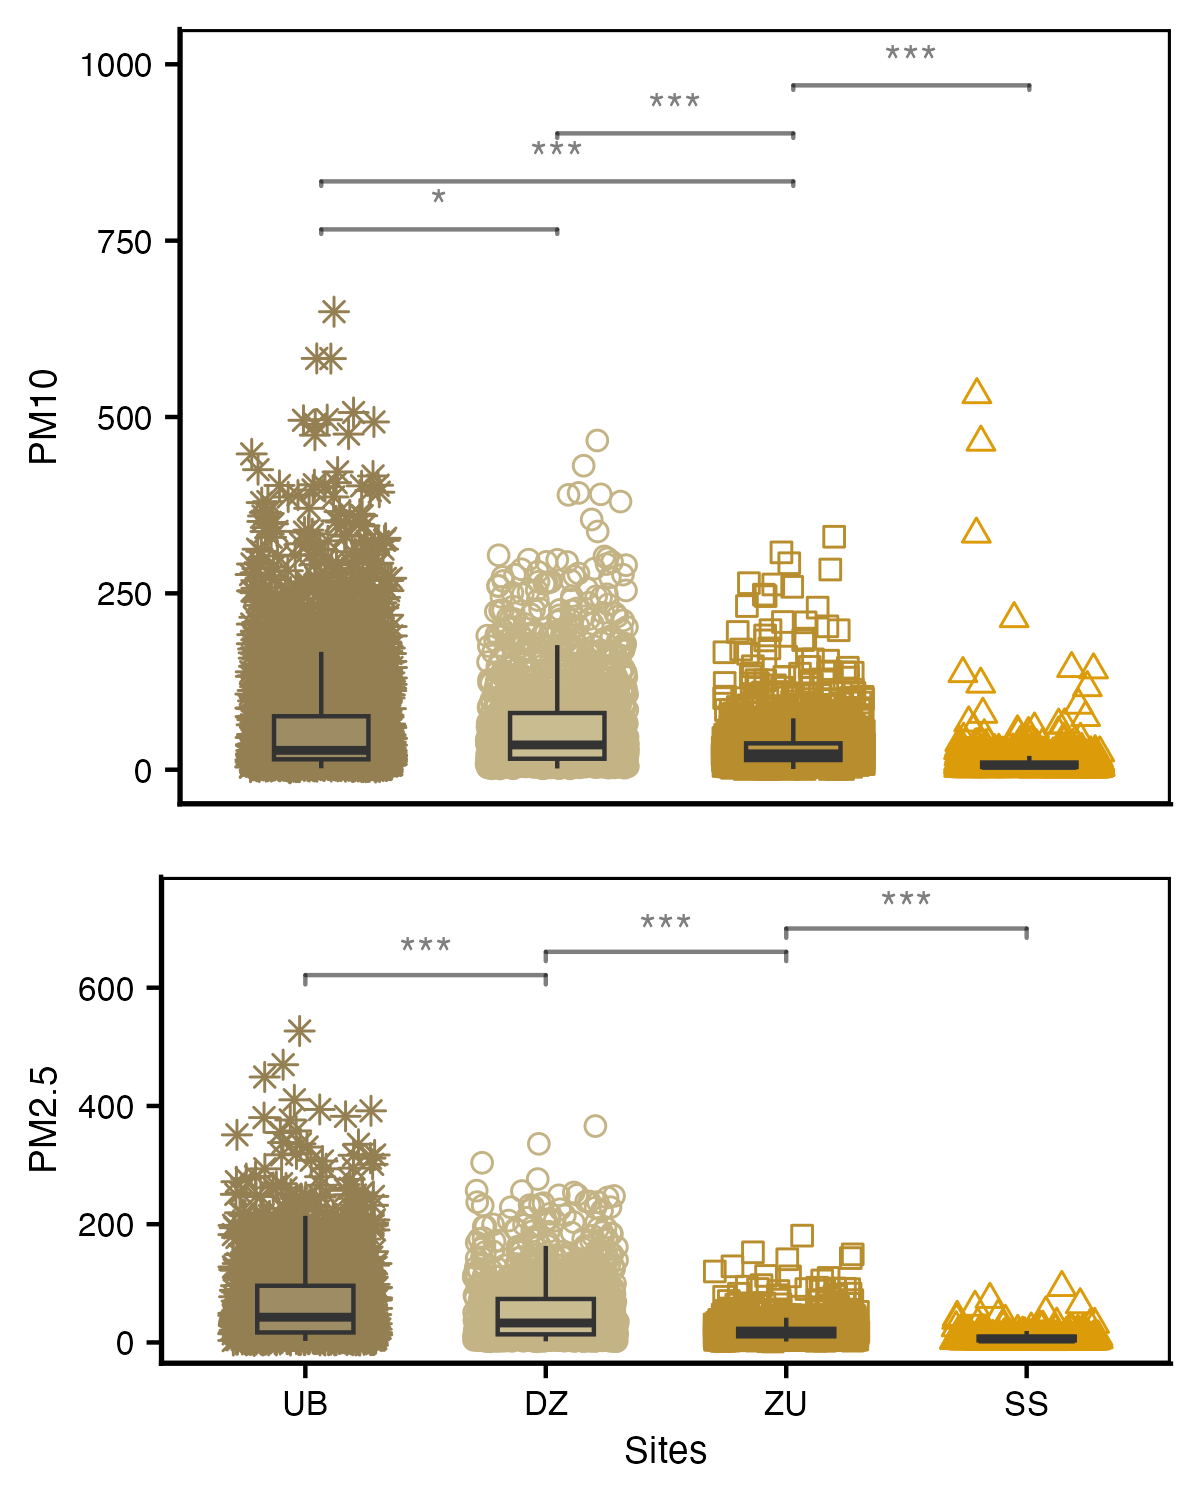
\includegraphics[width=3.125in,height=\textheight,keepaspectratio]{images/figure_3.png}
\caption{Distinct concentrations of coarse and fine particulates among
sites}
\end{figure}

\begin{enumerate}
\def\labelenumi{\arabic{enumi}.}
\tightlist
\item
  Compare the concentrations of PMs at UB is the 2. Significance level
  difference 3. Conclude
\end{enumerate}

\newpage

\begin{figure}
\centering
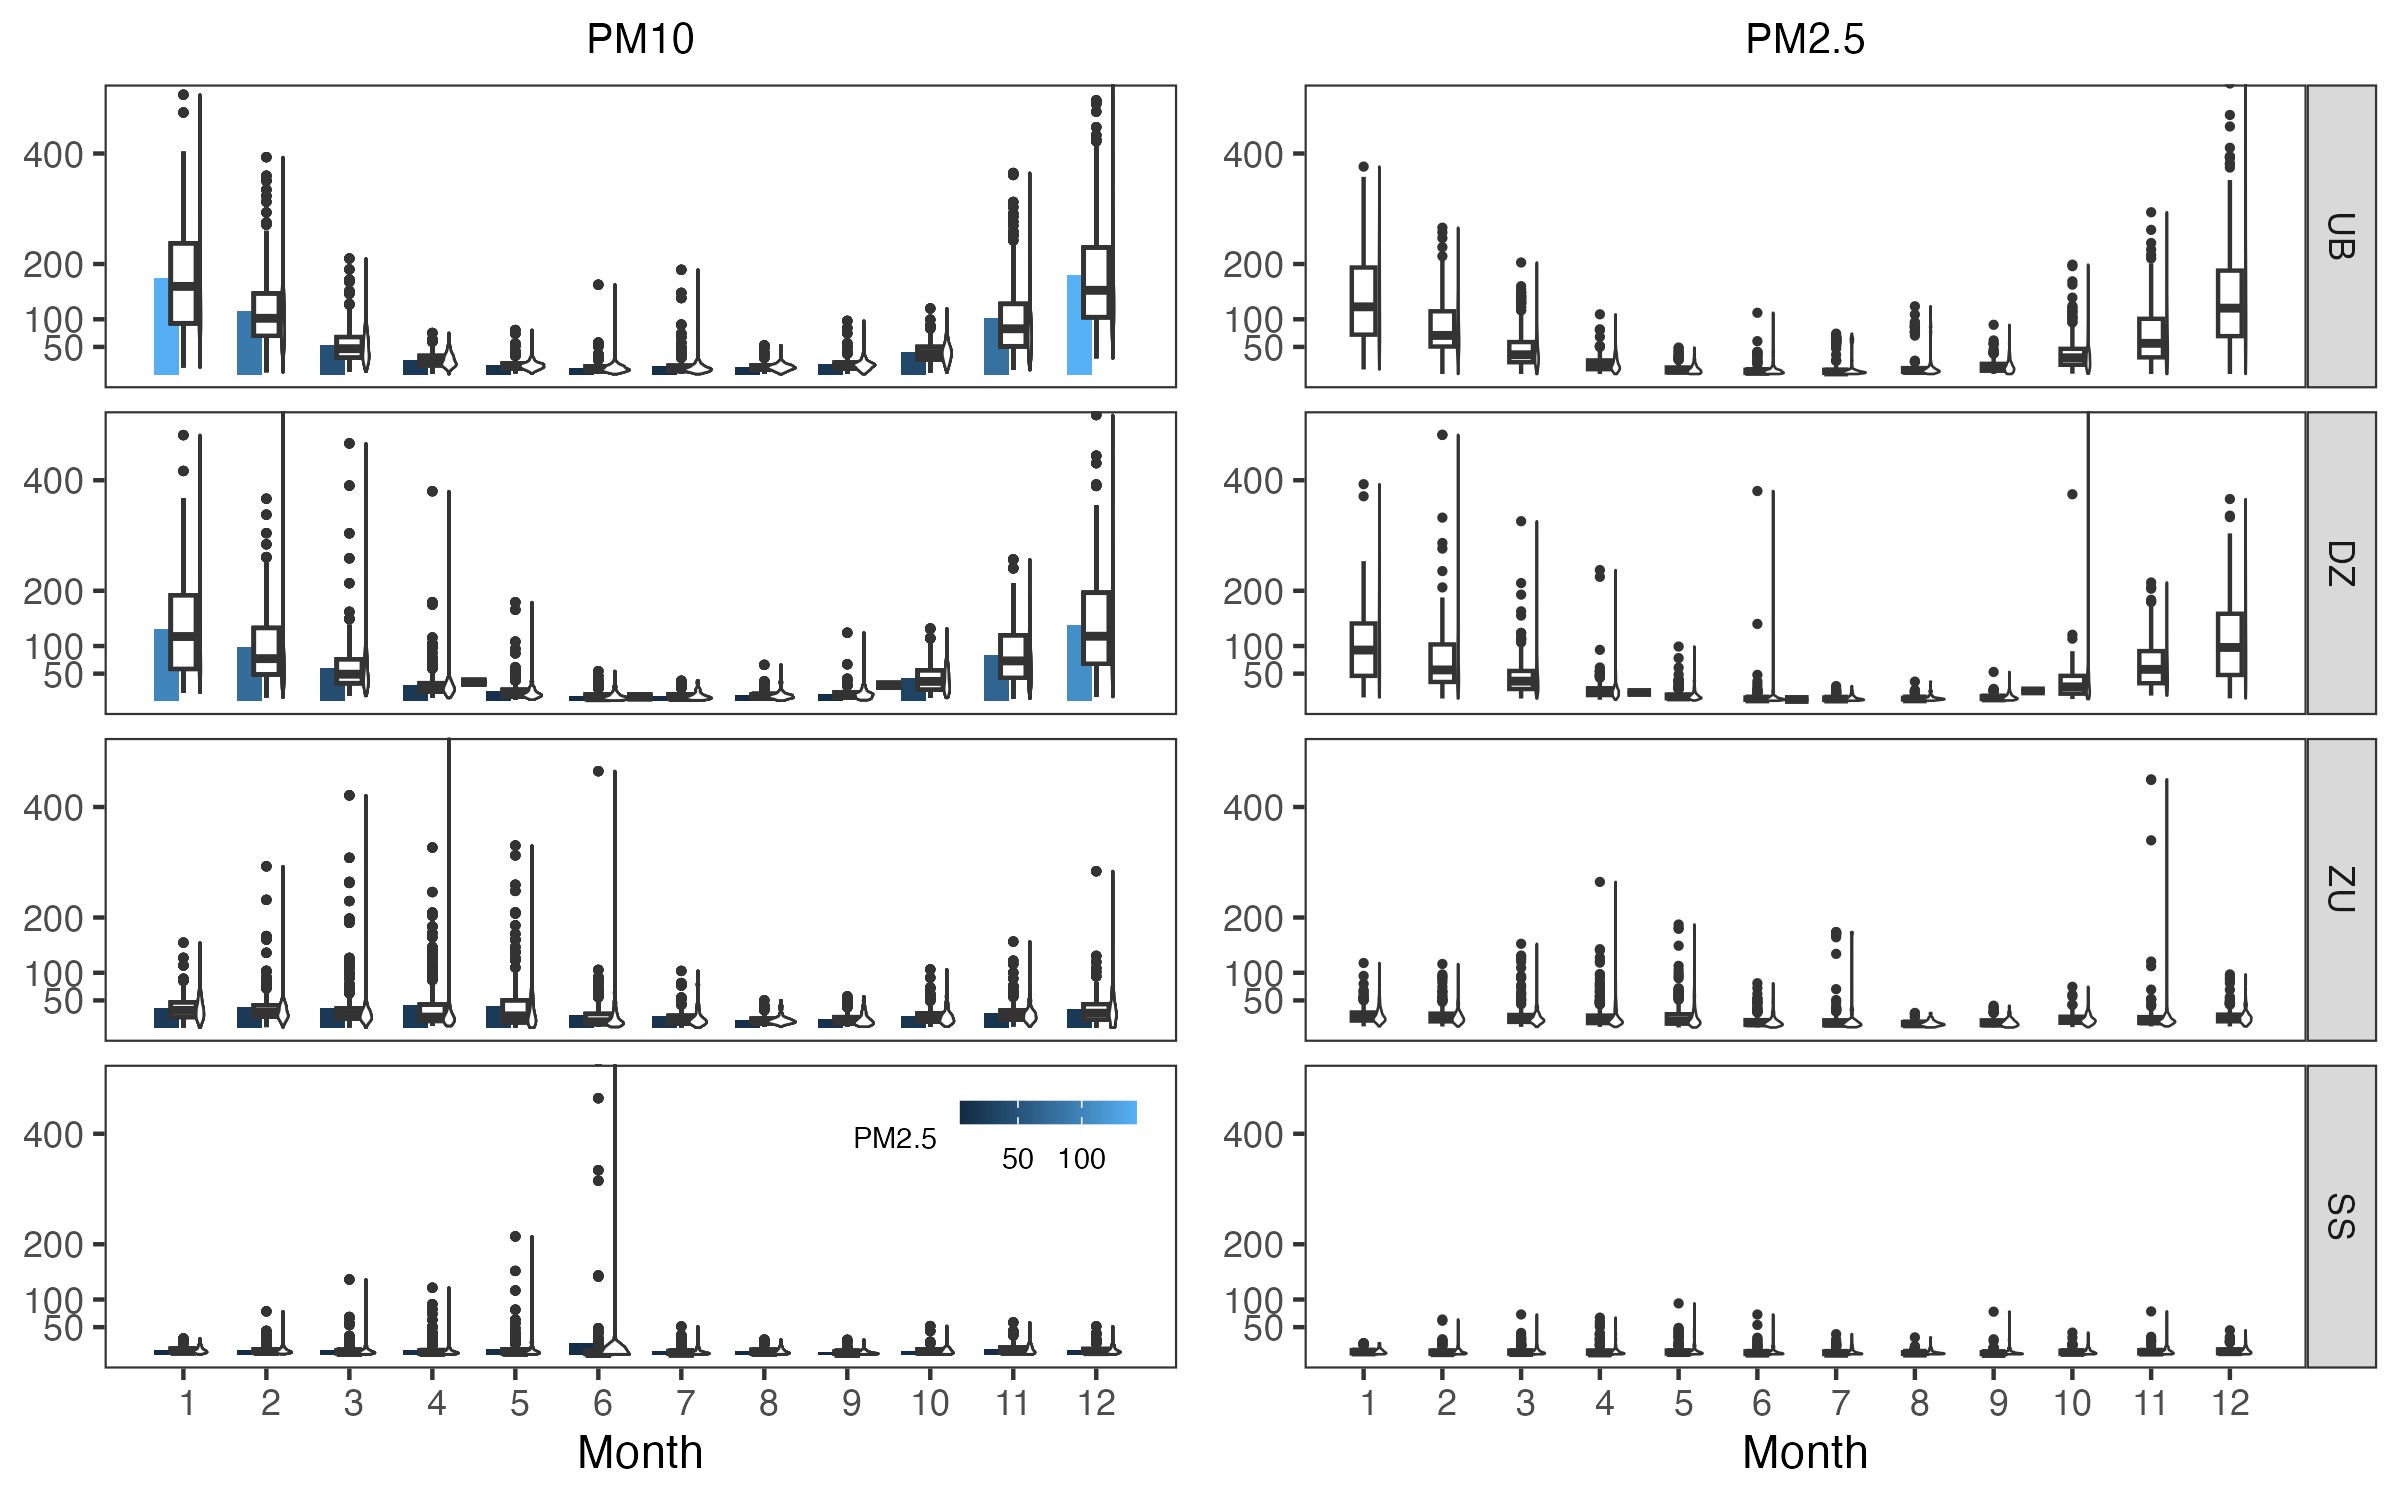
\includegraphics[width=3.4375in,height=\textheight,keepaspectratio]{images/figure_4.png}
\caption{Annual variations of \$PM\_\{10\}\$ and \$PM\_\{2.5\}\$}
\end{figure}

\begin{enumerate}
\def\labelenumi{\arabic{enumi}.}
\tightlist
\item
  Clear annual variations at UB and DZ from pm2.5 pollutions 2. at ZU,
  and SS has a seasonally peaks episodic spring and late autumn from
  PM10
\end{enumerate}

\newpage

\begin{figure}
\centering
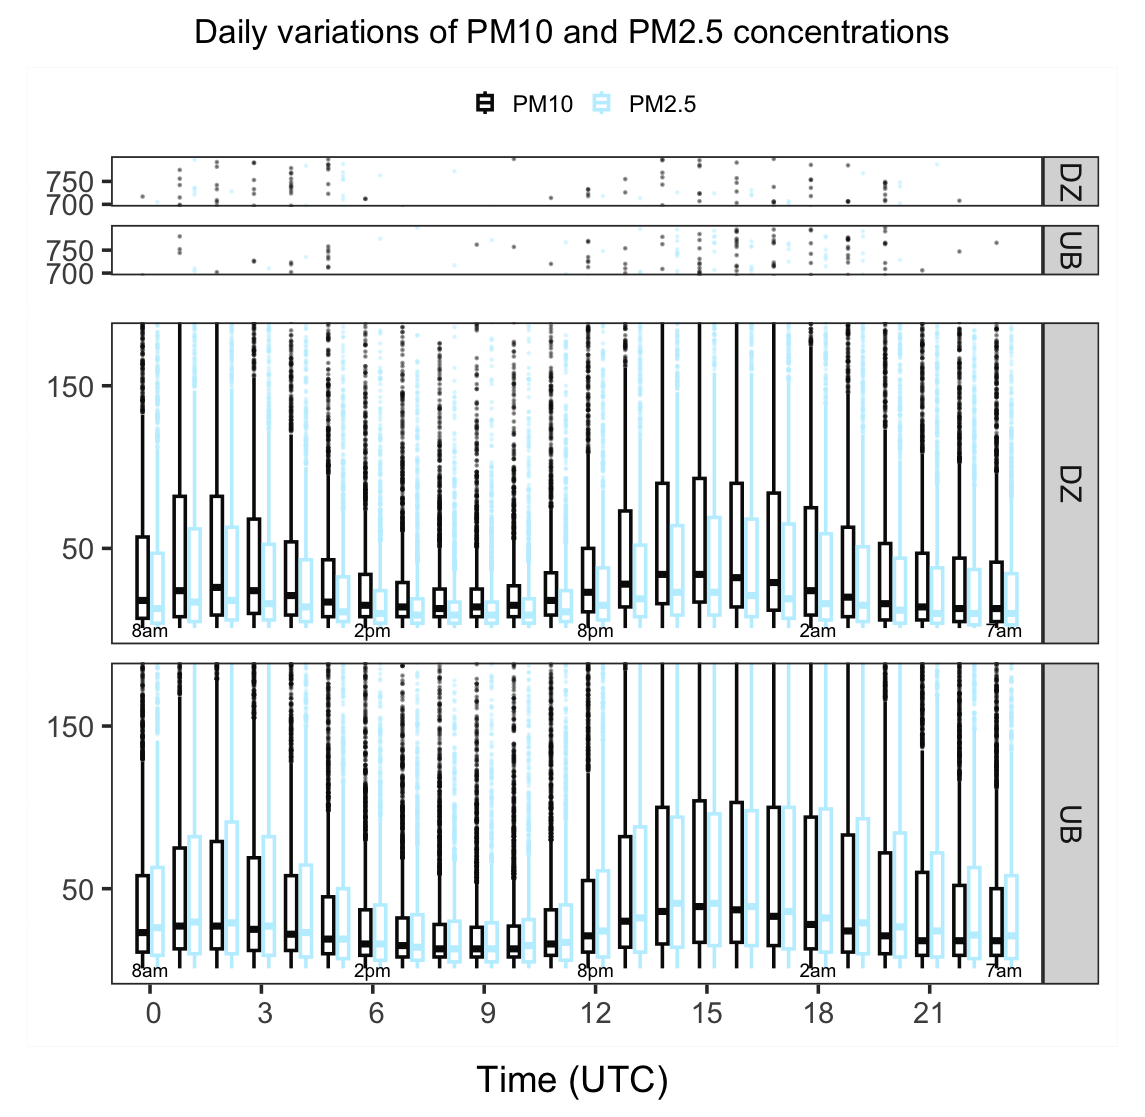
\includegraphics[width=3.125in,height=\textheight,keepaspectratio]{images/figure_5.png}
\caption{Daily variations of \(PM_{10}\) and \(PM_{2.5}\) at UB and DZ
sites}
\end{figure}

\newpage
\subsection{Meteorological influence on $PM_{10}$ and $PM_{2.5}$ variations}
\label{subsec2}

\begin{figure}
\centering
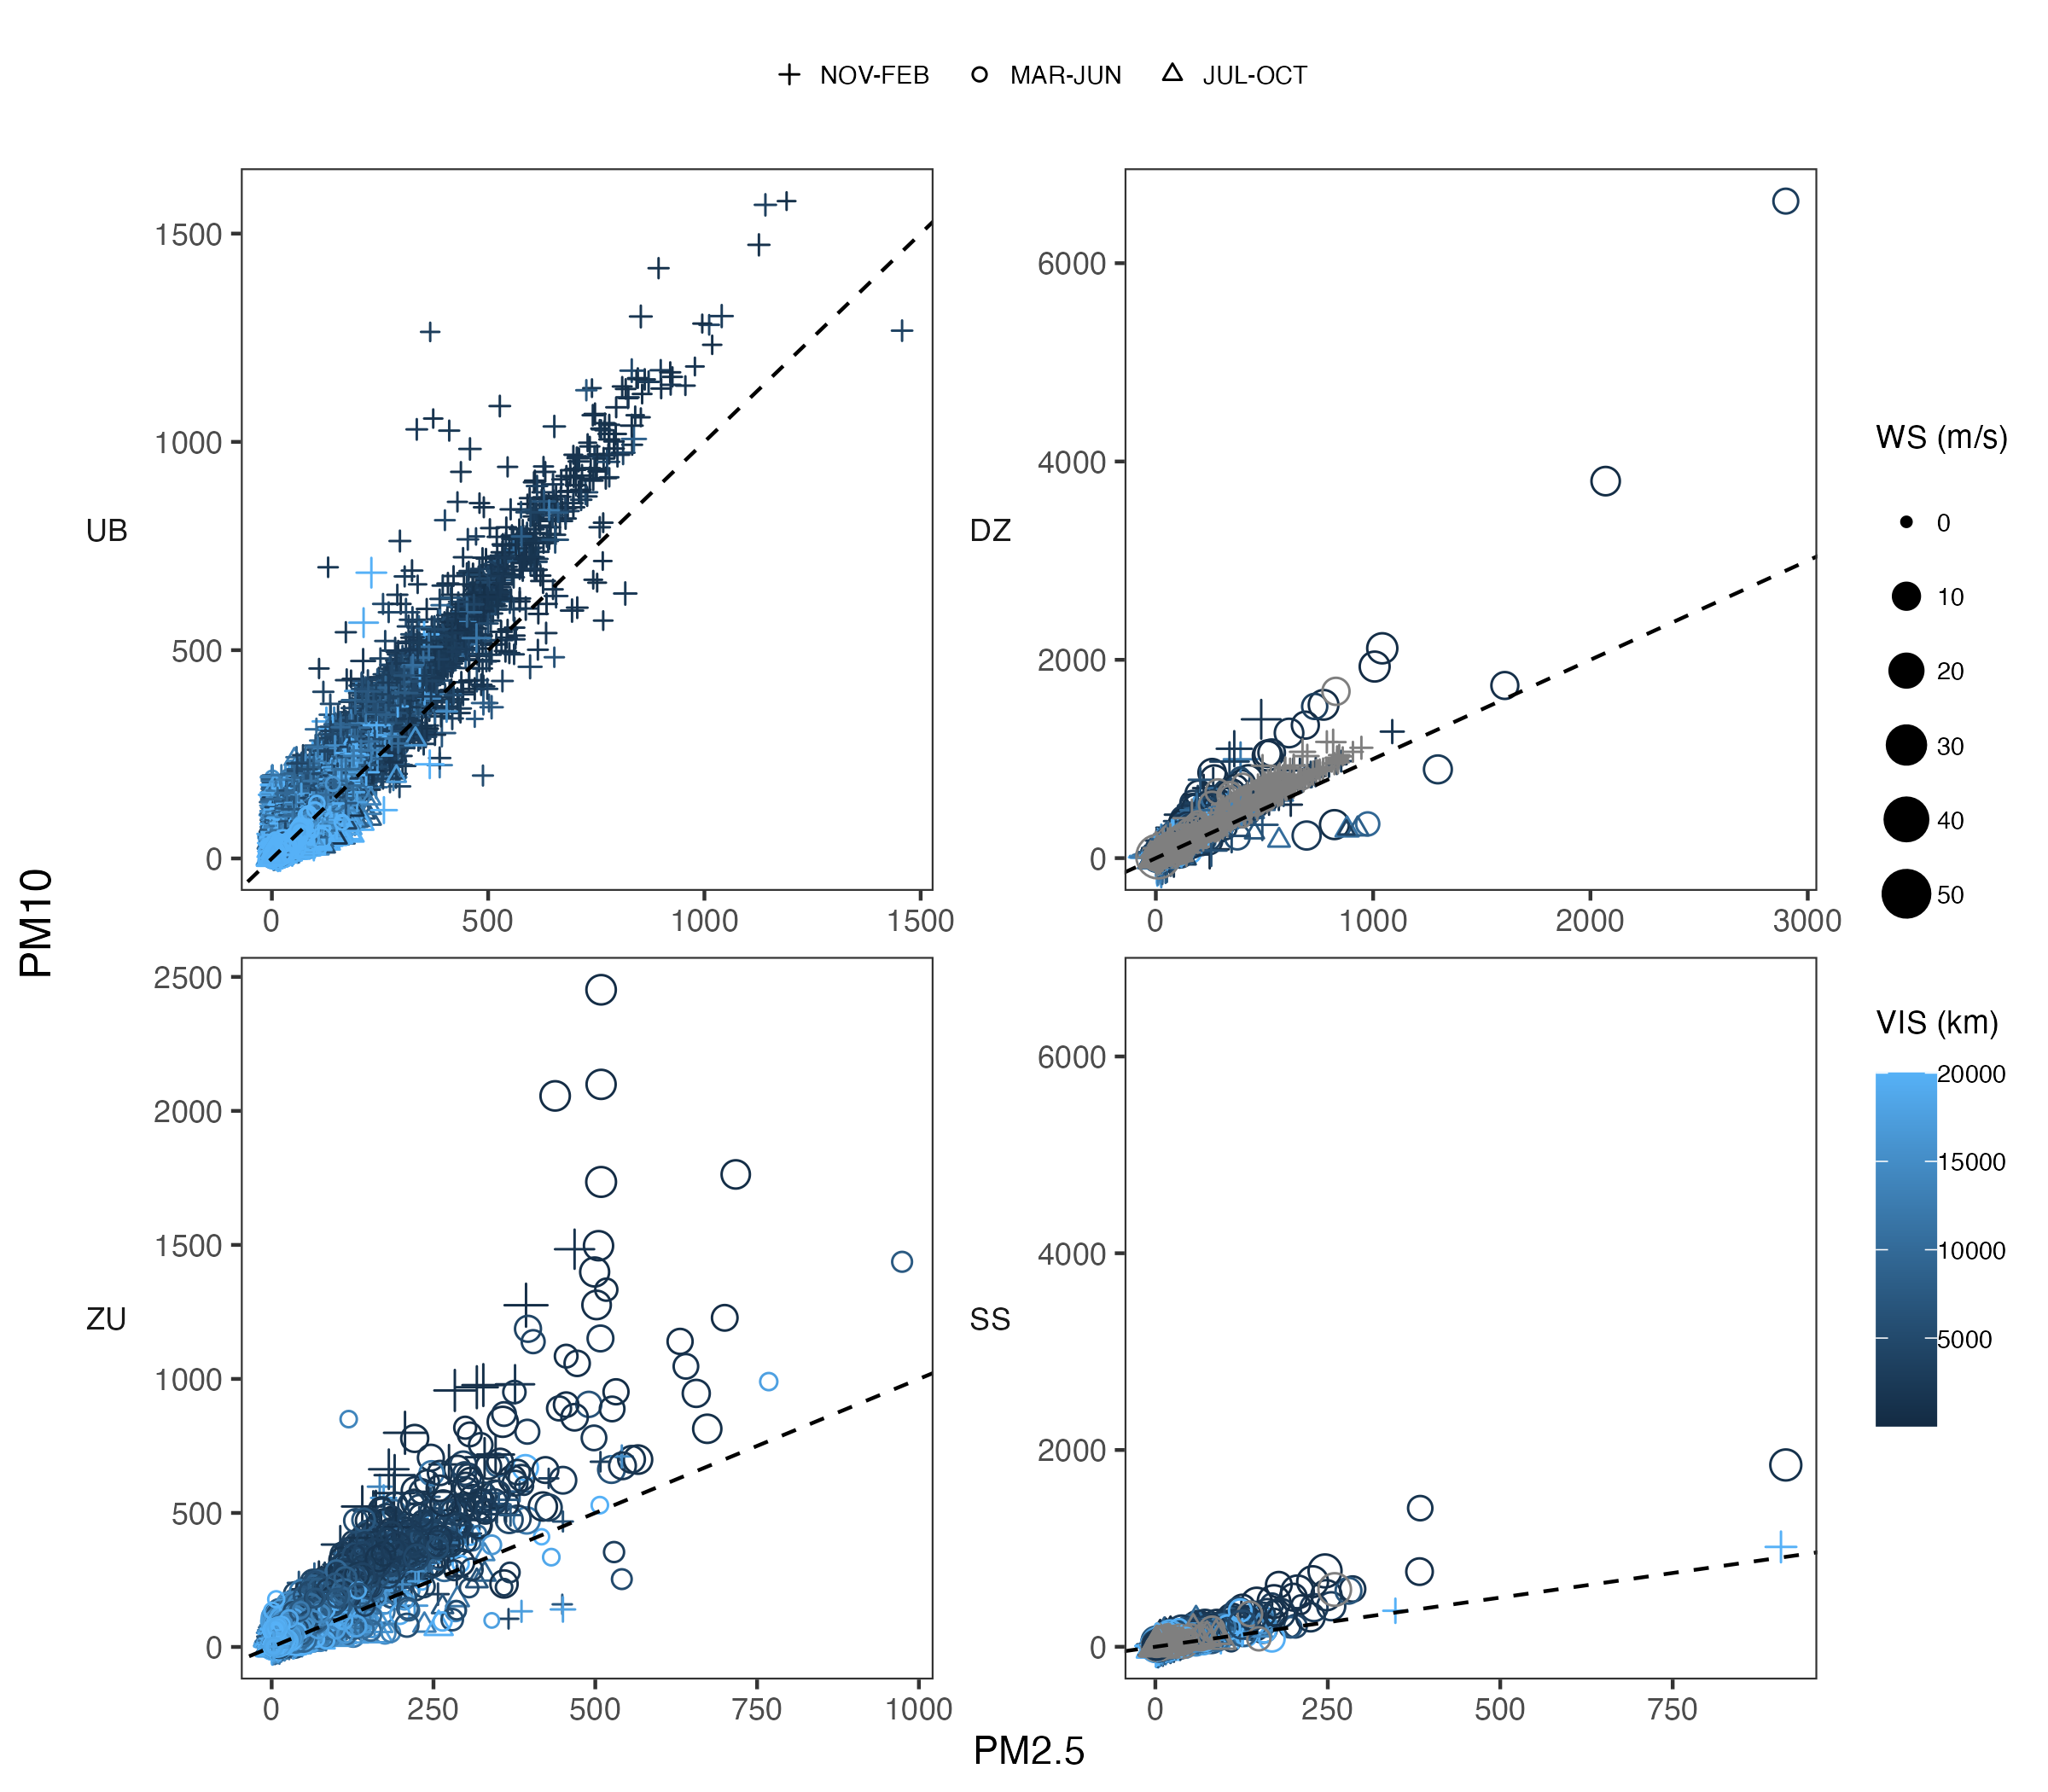
\includegraphics[width=3.125in,height=\textheight,keepaspectratio]{images/figure_6.png}
\caption{Relationships between meteorological major factors and
variations of \(PM_{10}\) and \(PM_{2.5}\)}
\end{figure}

\newpage

\begin{figure}
\centering
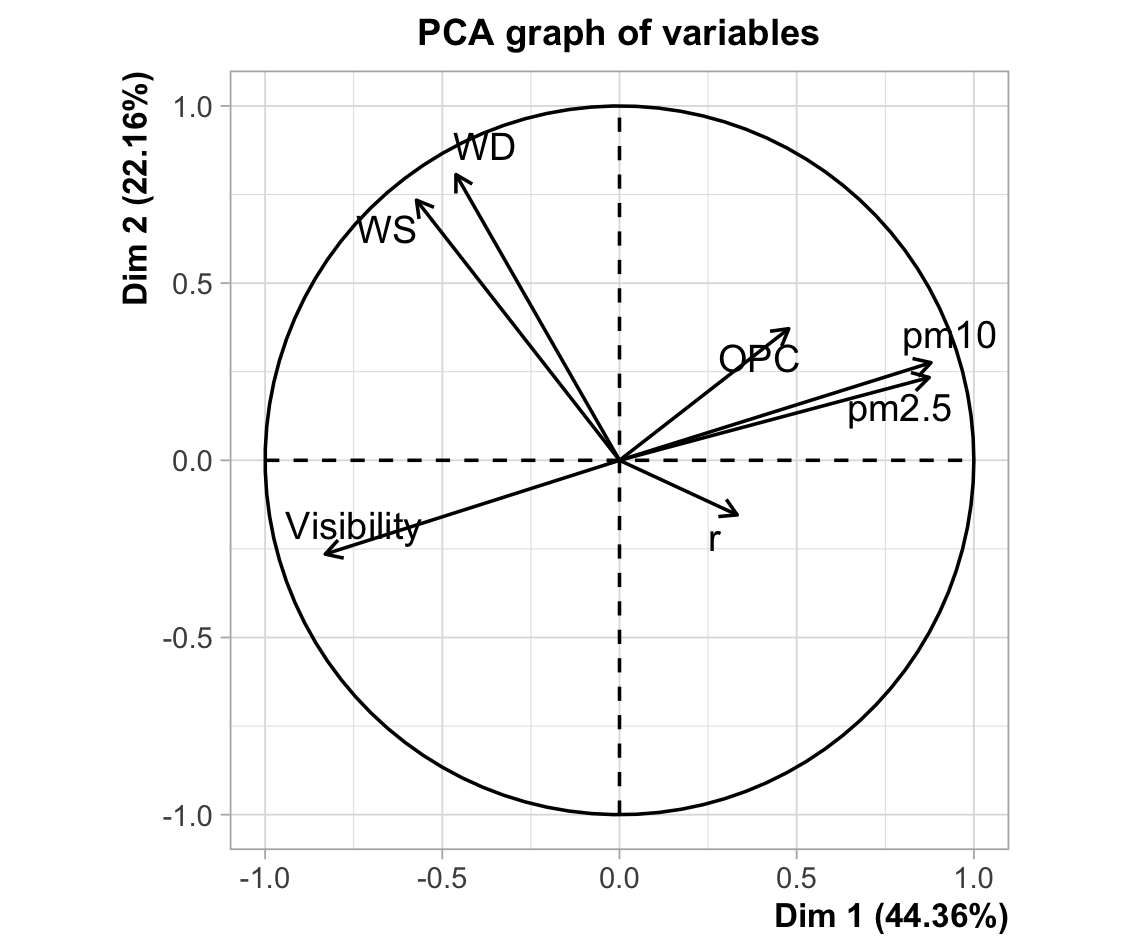
\includegraphics[width=2.08333in,height=\textheight,keepaspectratio]{images/figure_7.png}
\caption{Spatio-temporal distinct feature of variations of \(PM_{10}\)
and \(PM_{2.5}\) with PCA analysis}
\end{figure}

\begin{figure}
\centering
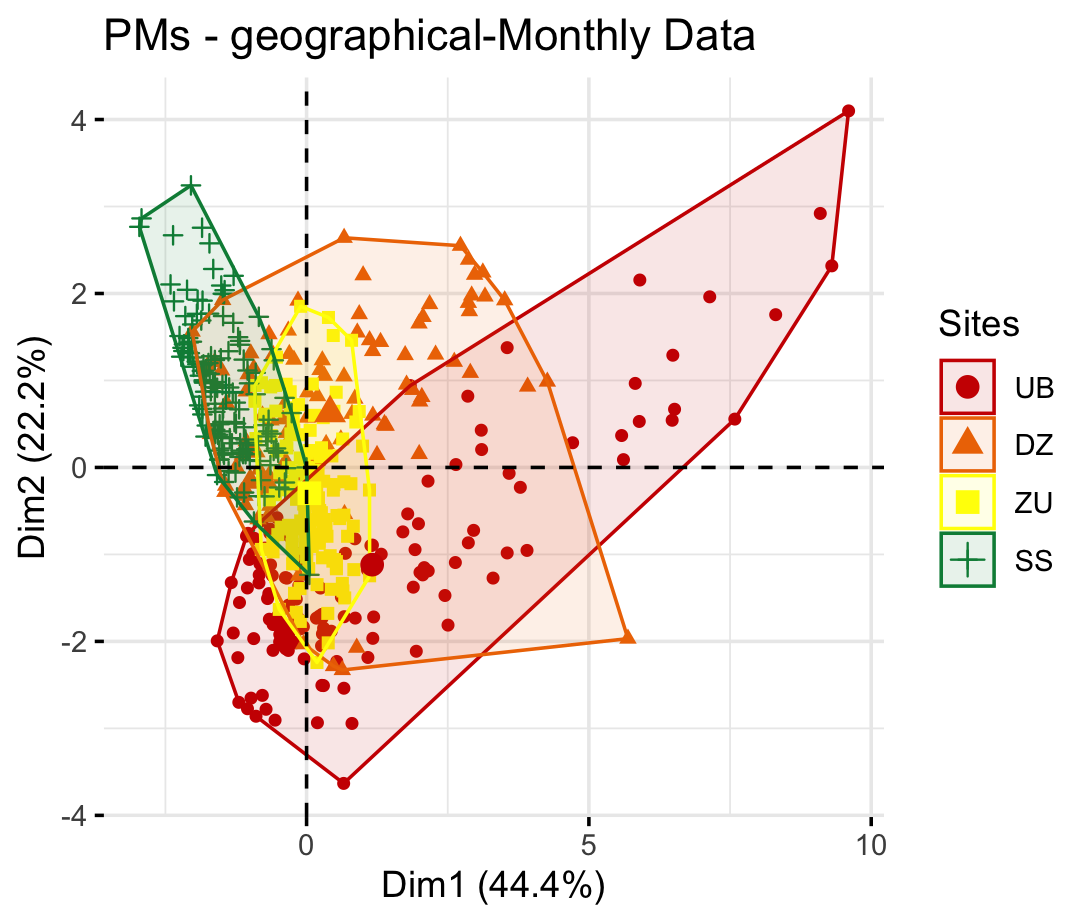
\includegraphics[width=2.08333in,height=\textheight,keepaspectratio]{images/figure_7b.png}
\caption{Patterns of meteorology and PMs at the 4 sites}
\end{figure}

\newpage
\subsection{Trends}

\begin{figure}
\centering
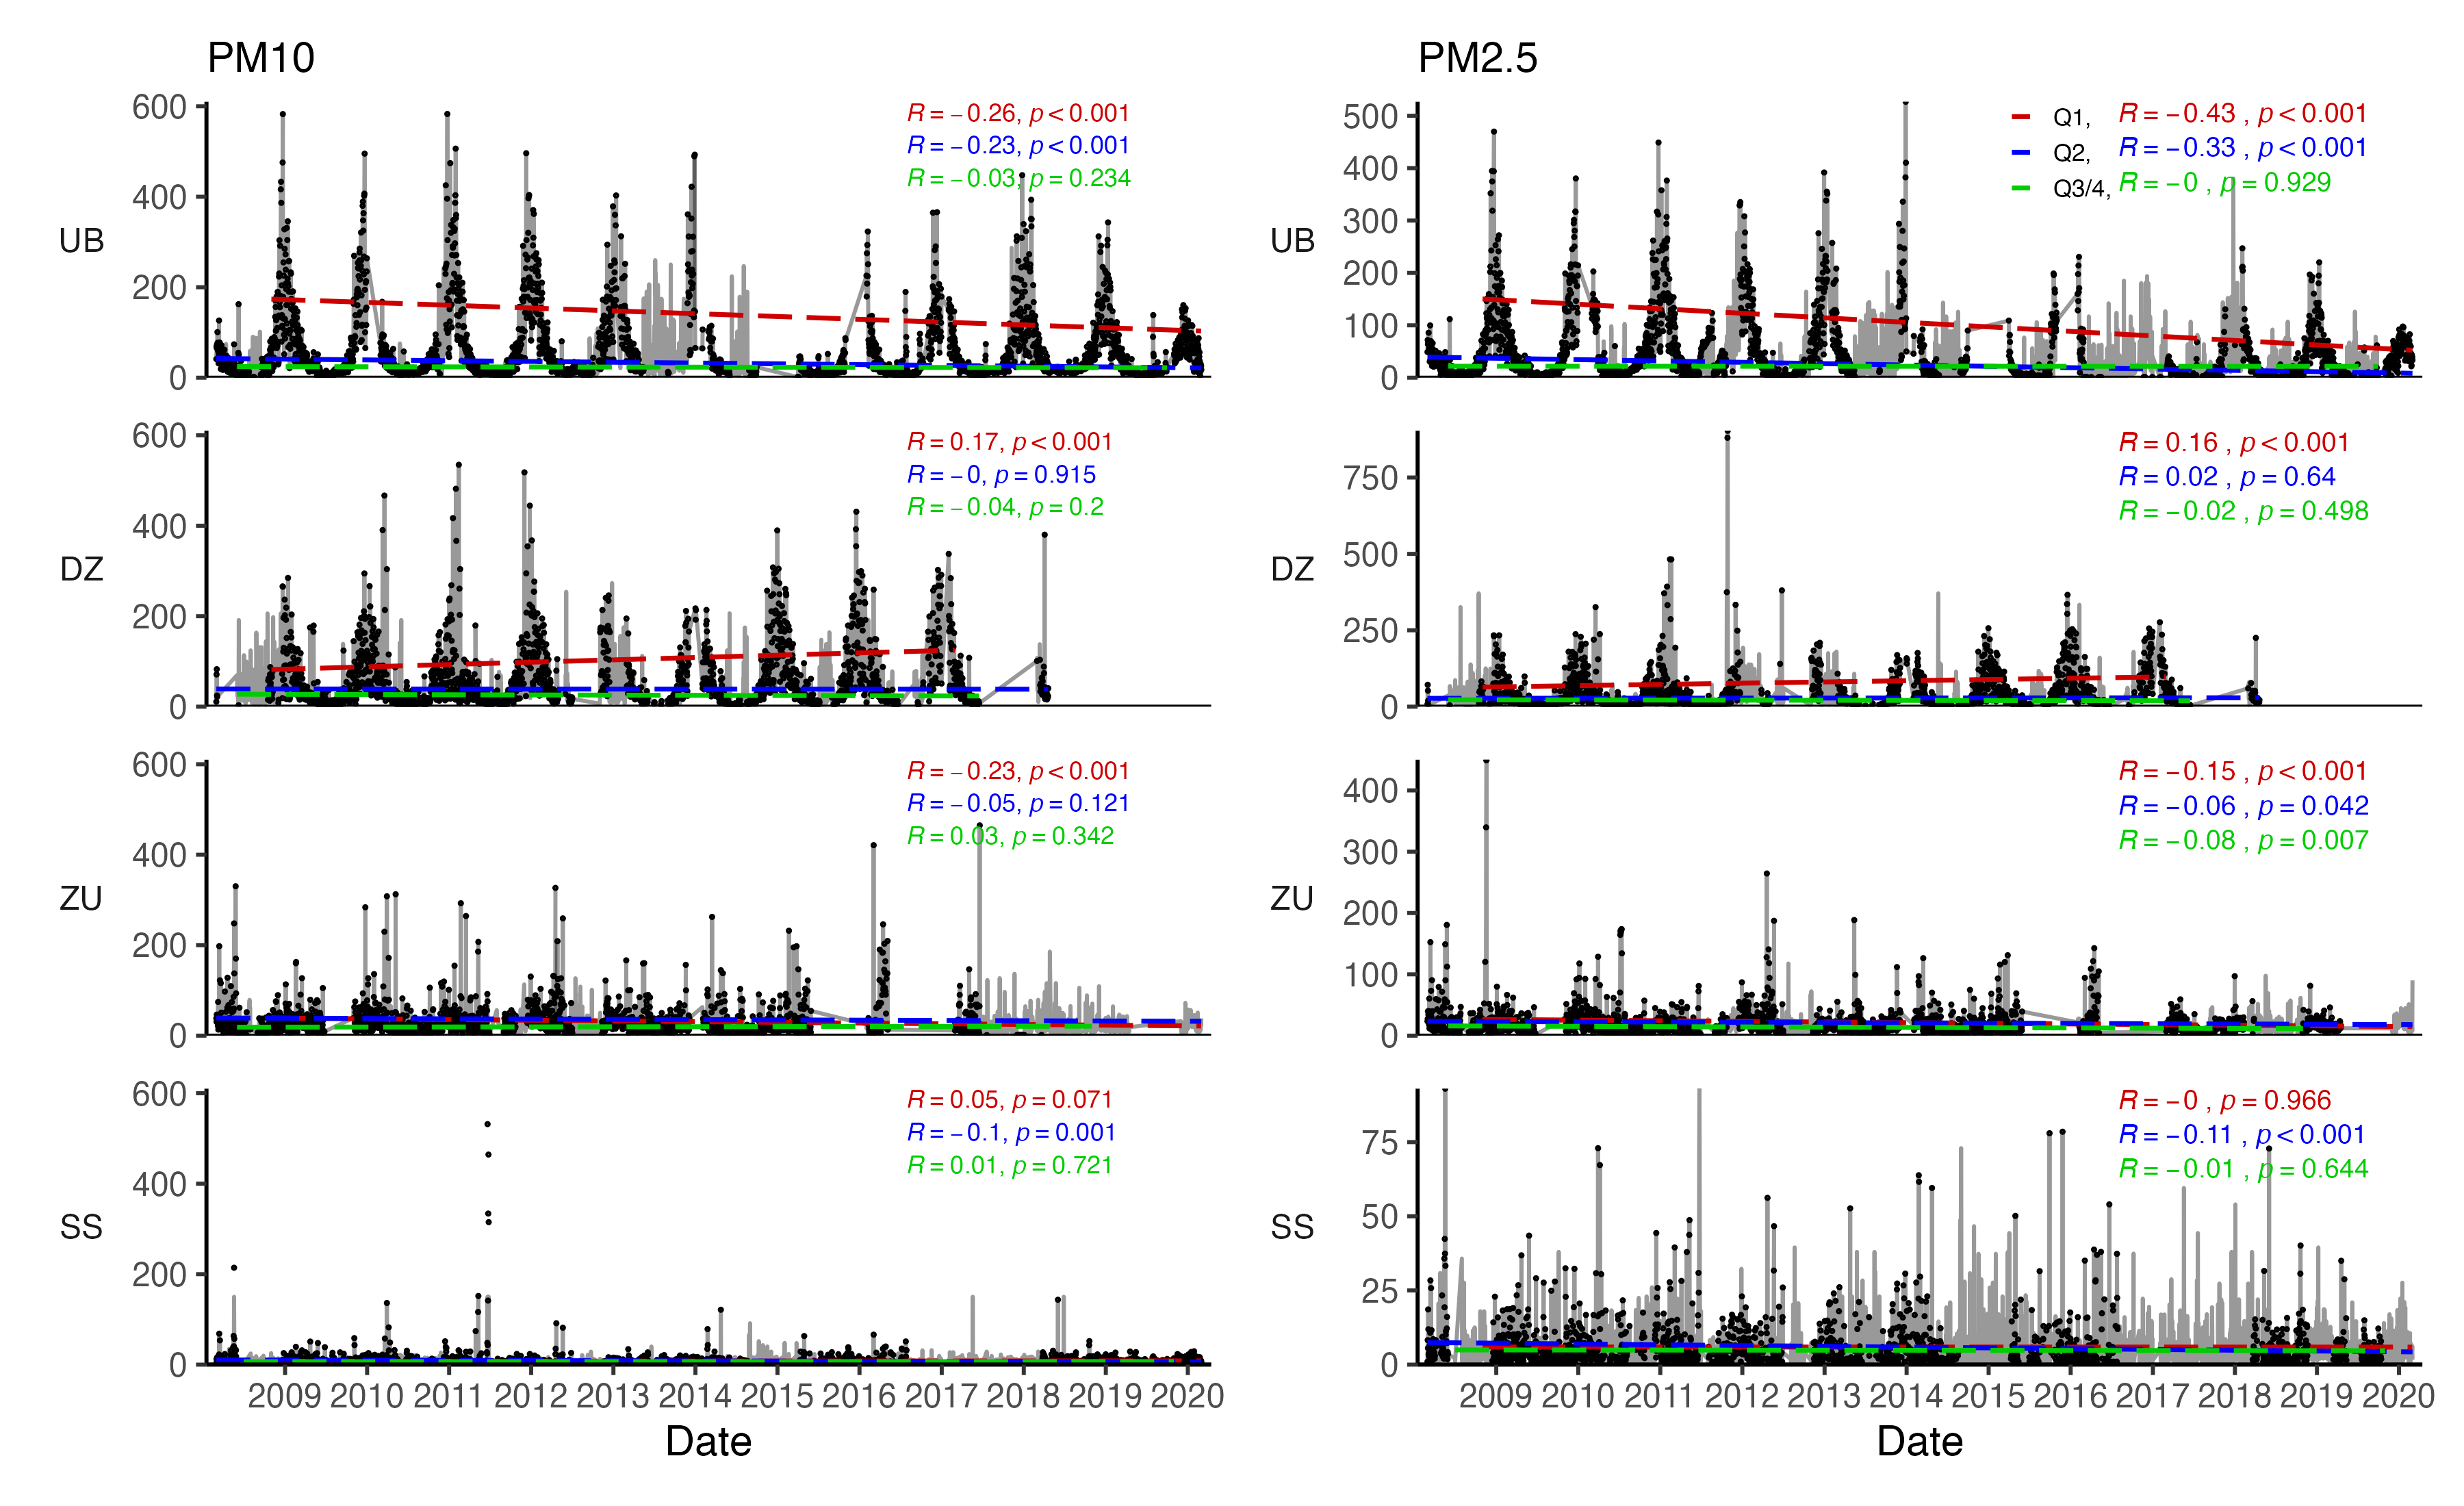
\includegraphics[width=3.125in,height=\textheight,keepaspectratio]{images/figure_8.png}
\caption{Interannual and seasonal trends of \(PM_{10}\) and \(PM_{2.5}\)
variations}
\end{figure}

\newpage

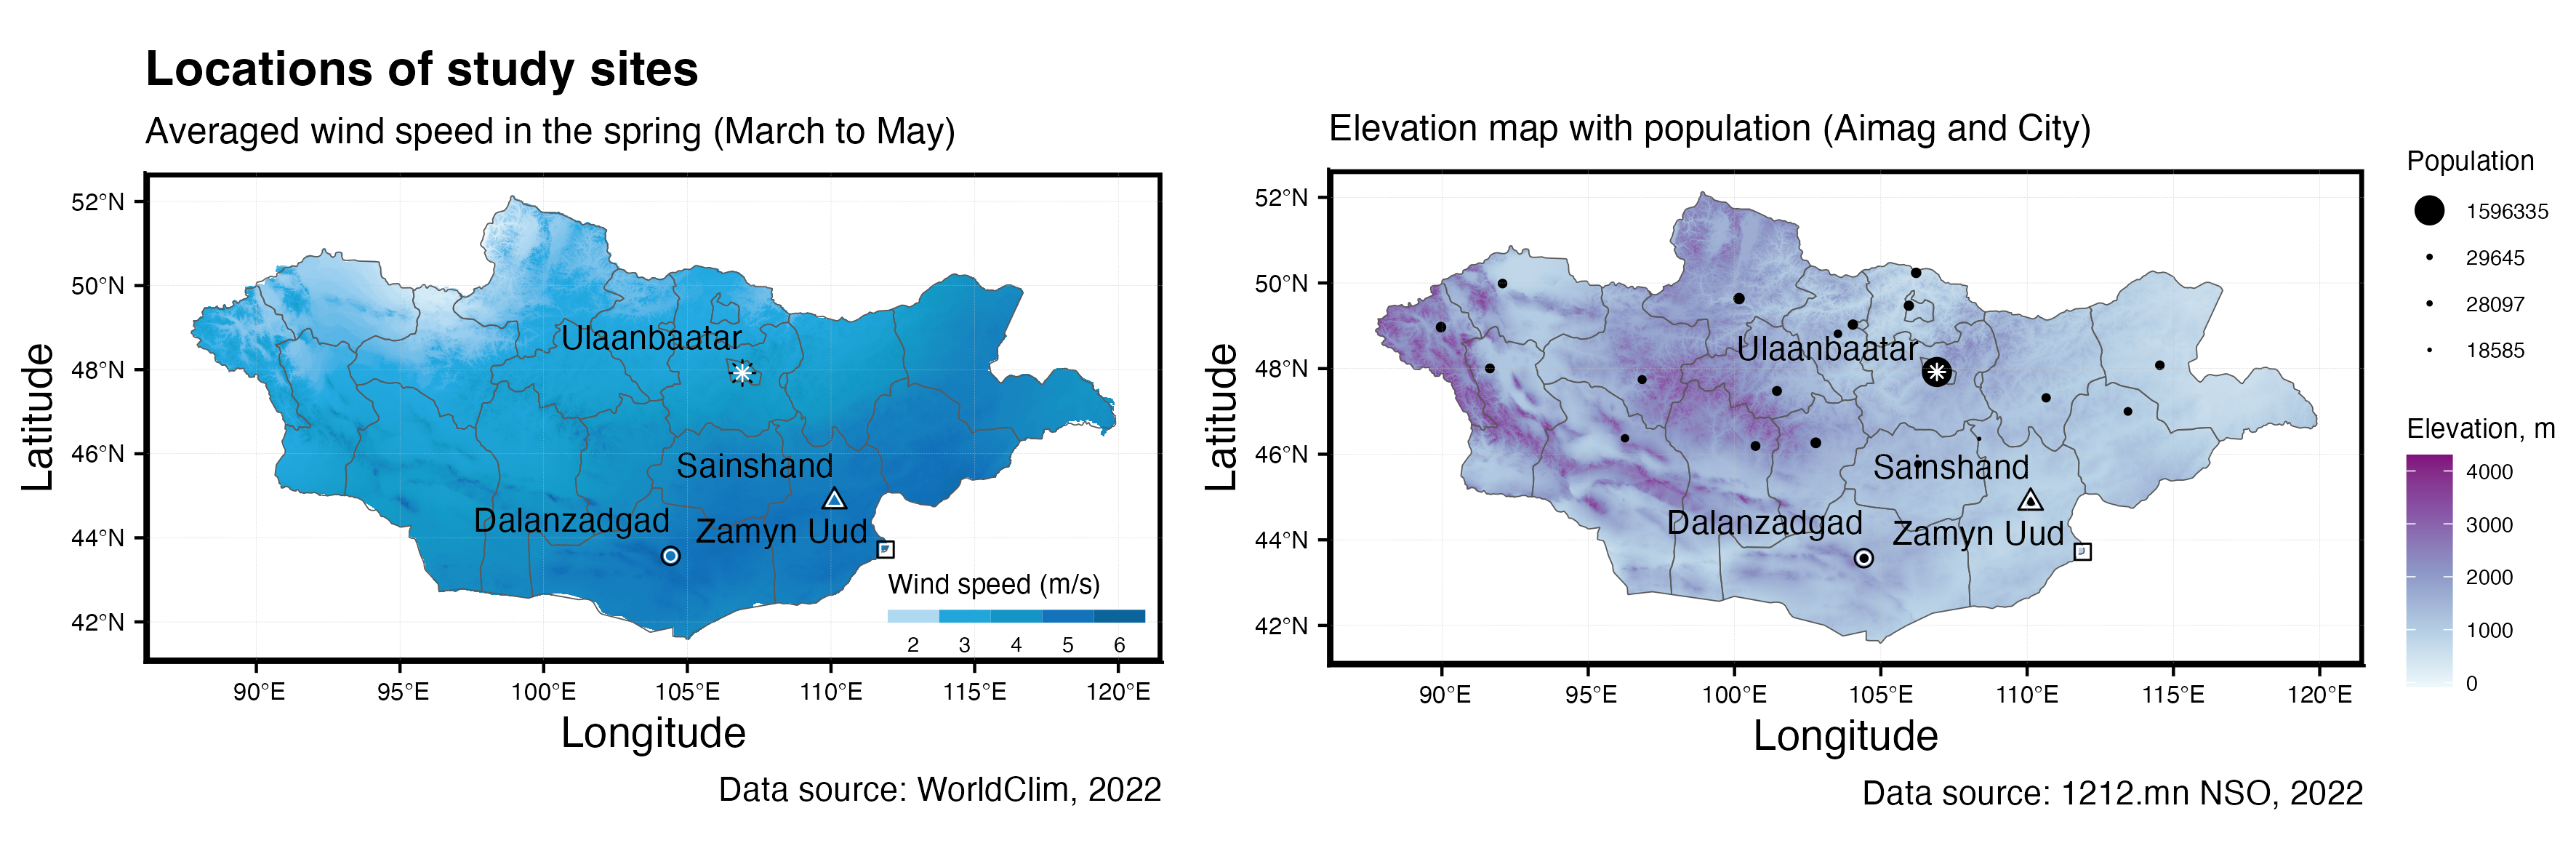
\includegraphics[width=3.125in,height=\textheight,keepaspectratio]{images/figure_1.png}{]}

\begin{figure}
\centering
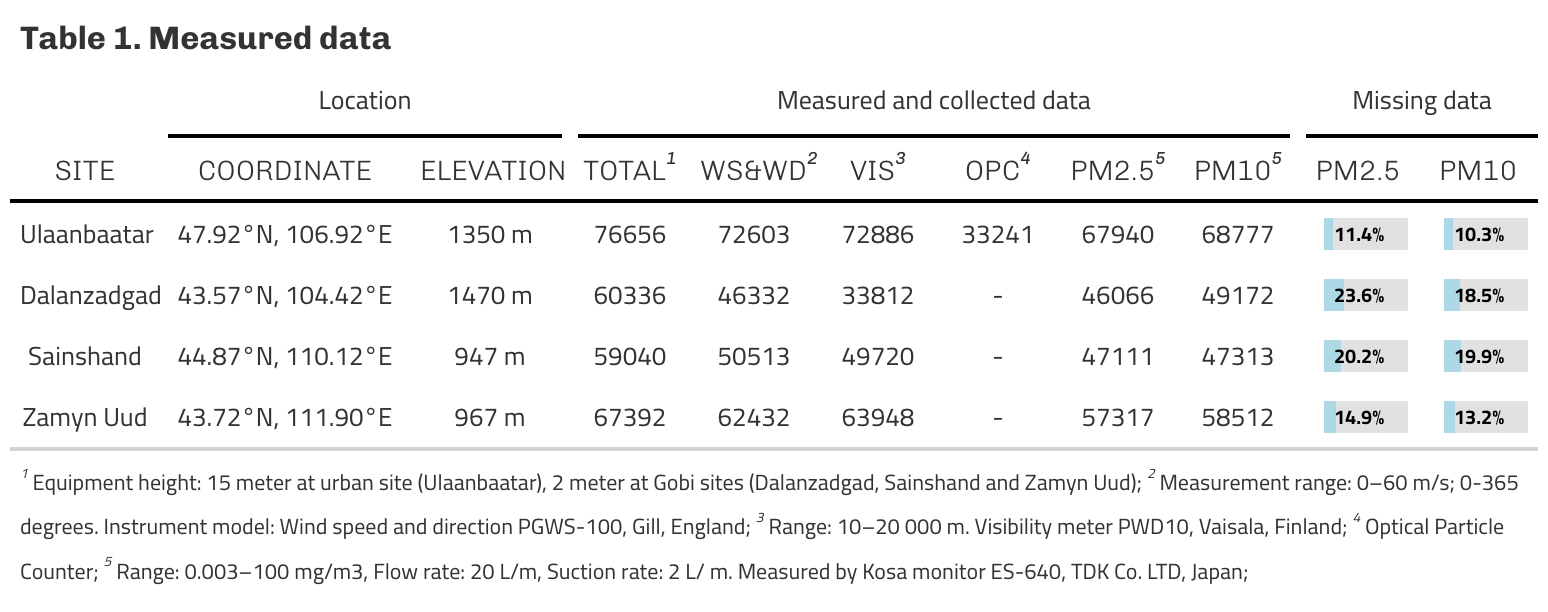
\includegraphics[width=4.16667in,height=\textheight,keepaspectratio]{images/table_1.png}
\caption{\textbf{Table 1}. A description of datasets obtained at the
sites}
\end{figure}

\newpage

\begin{figure}
\centering
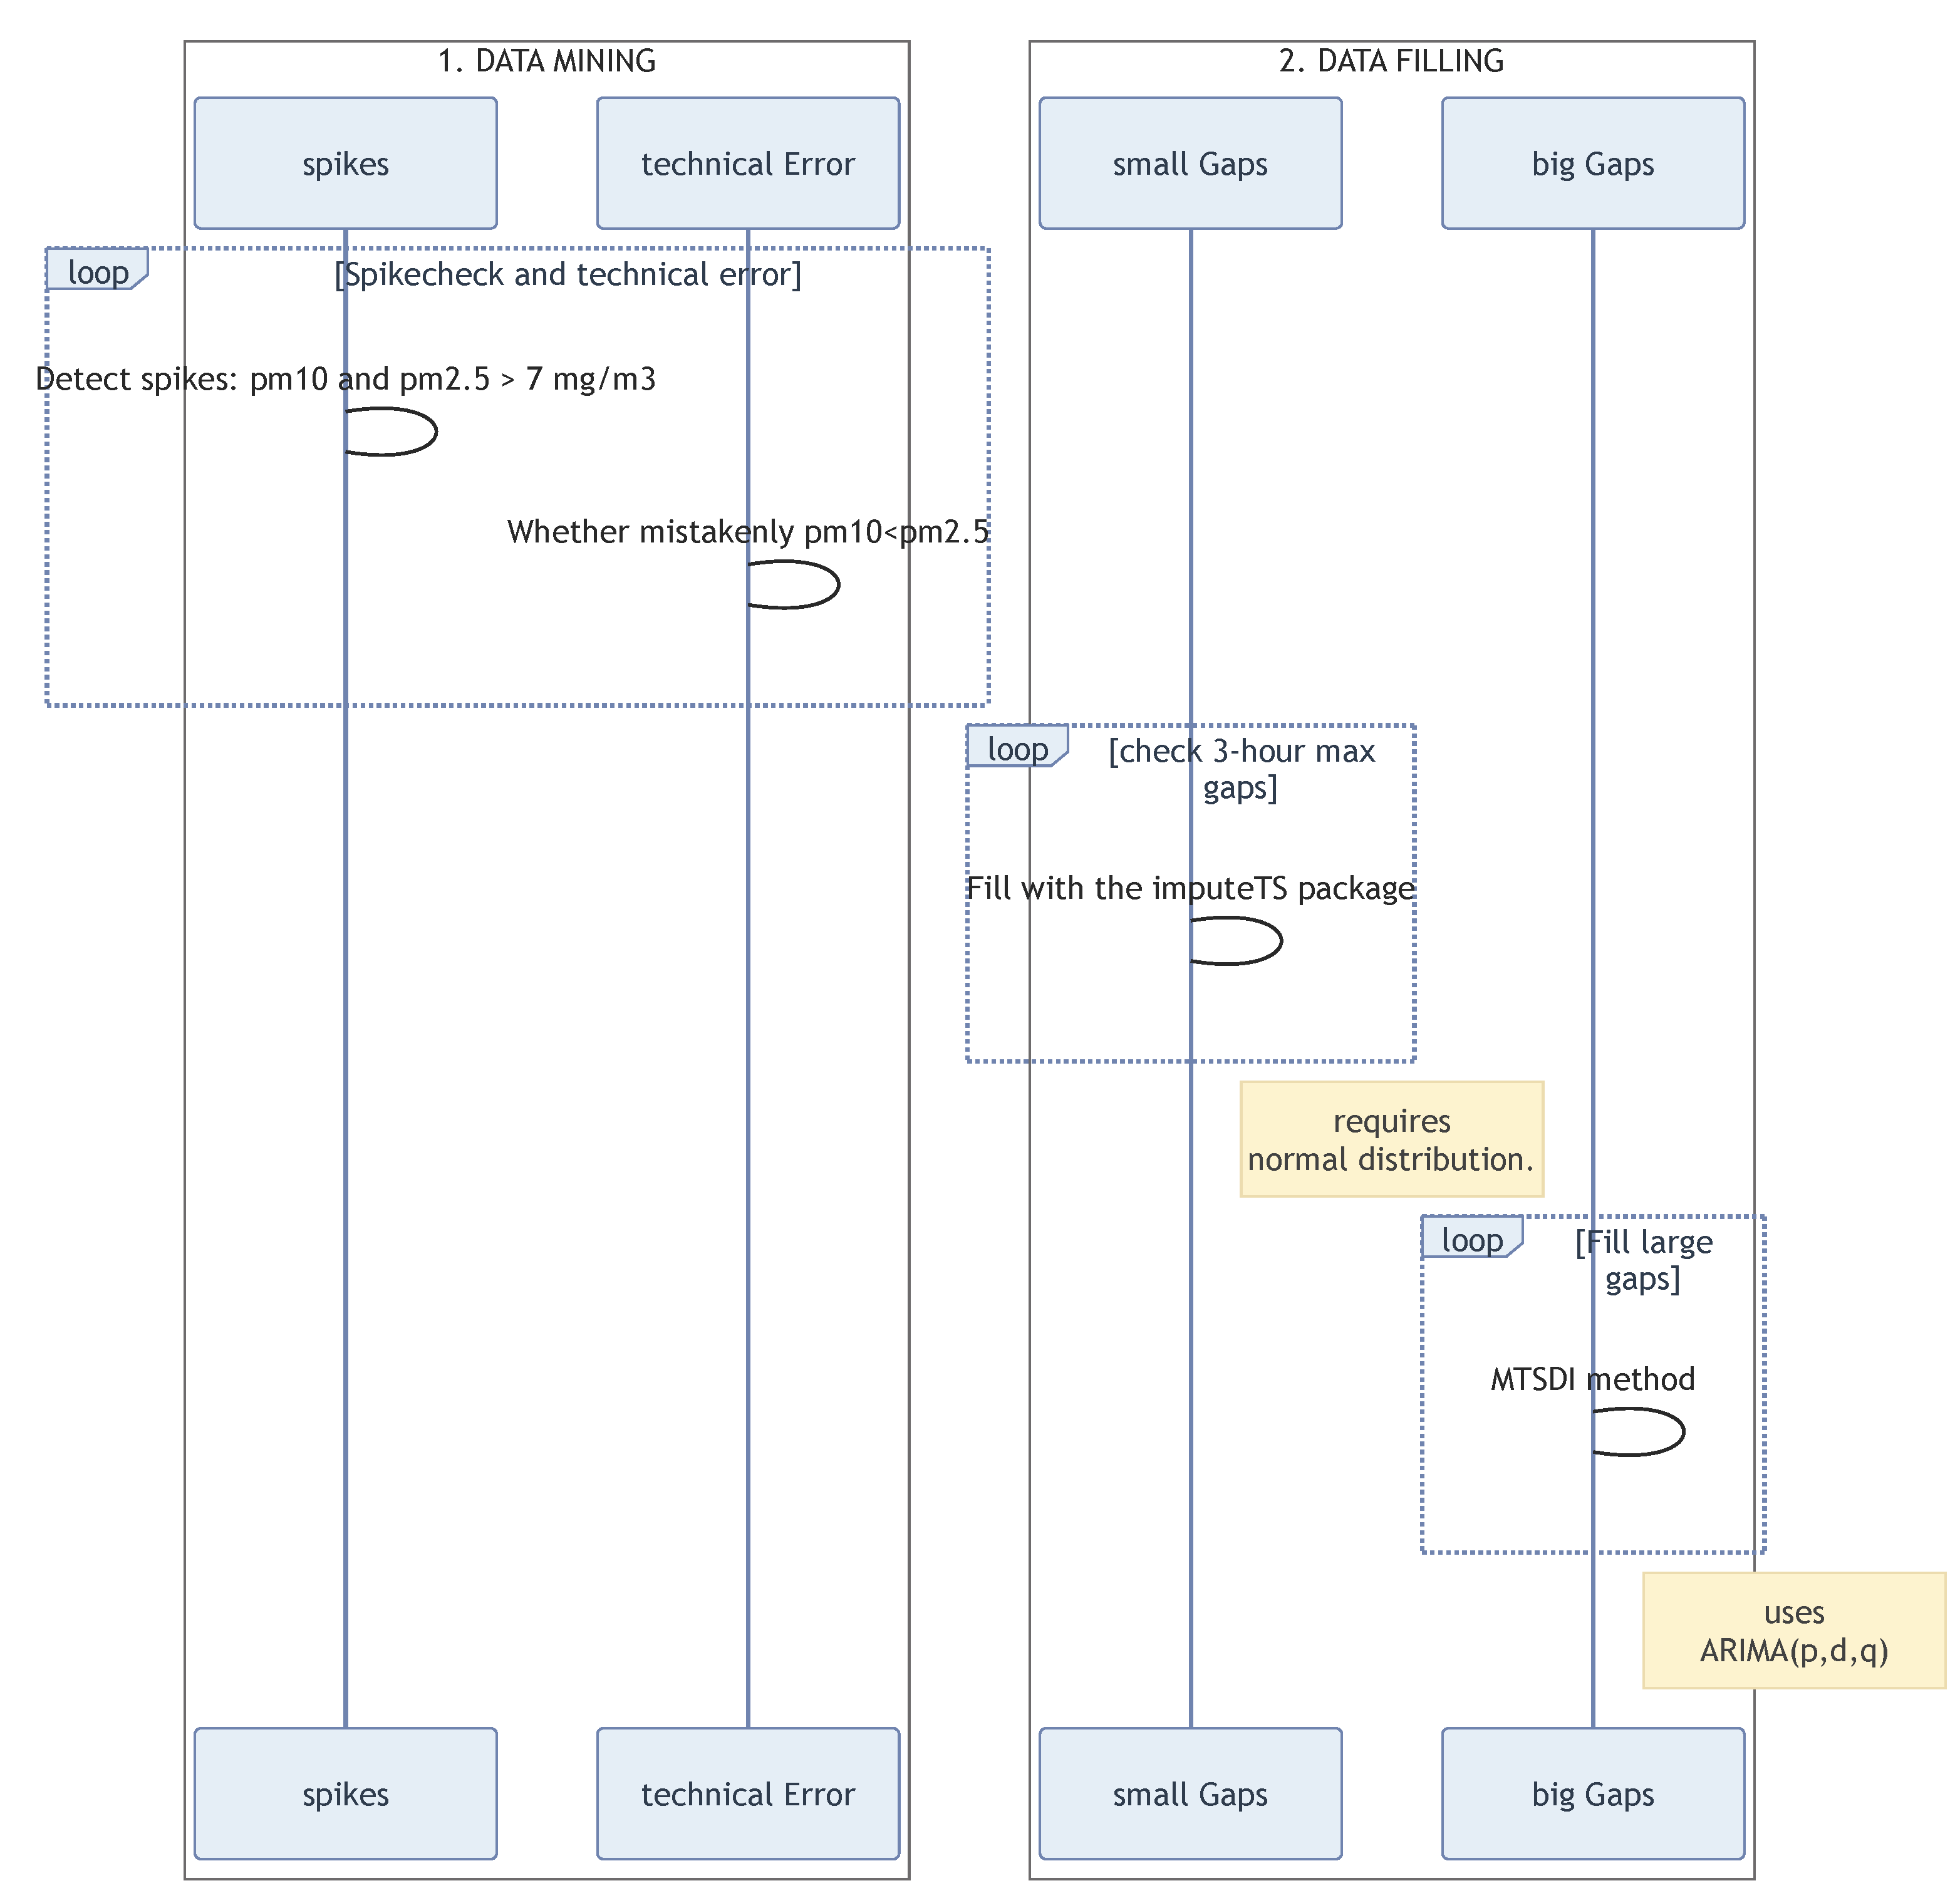
\includegraphics[width=3.125in,height=\textheight,keepaspectratio]{images/scheme_1.png}
\caption{Scheme 1. Data handling procedure}
\end{figure}

\newpage

\begin{figure}
\centering
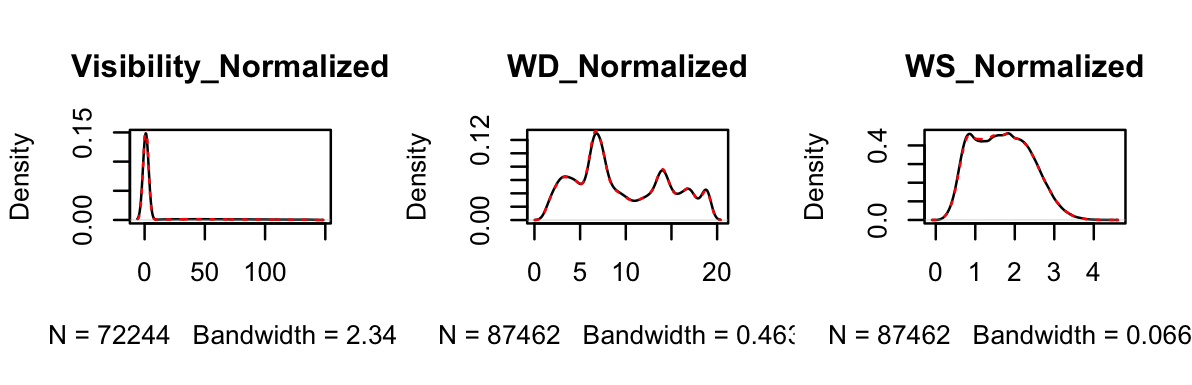
\includegraphics[width=3.125in,height=\textheight,keepaspectratio]{images/figure_2b.png}
\caption{Figure 2. Data gap filling}
\end{figure}

\begin{figure}
\centering
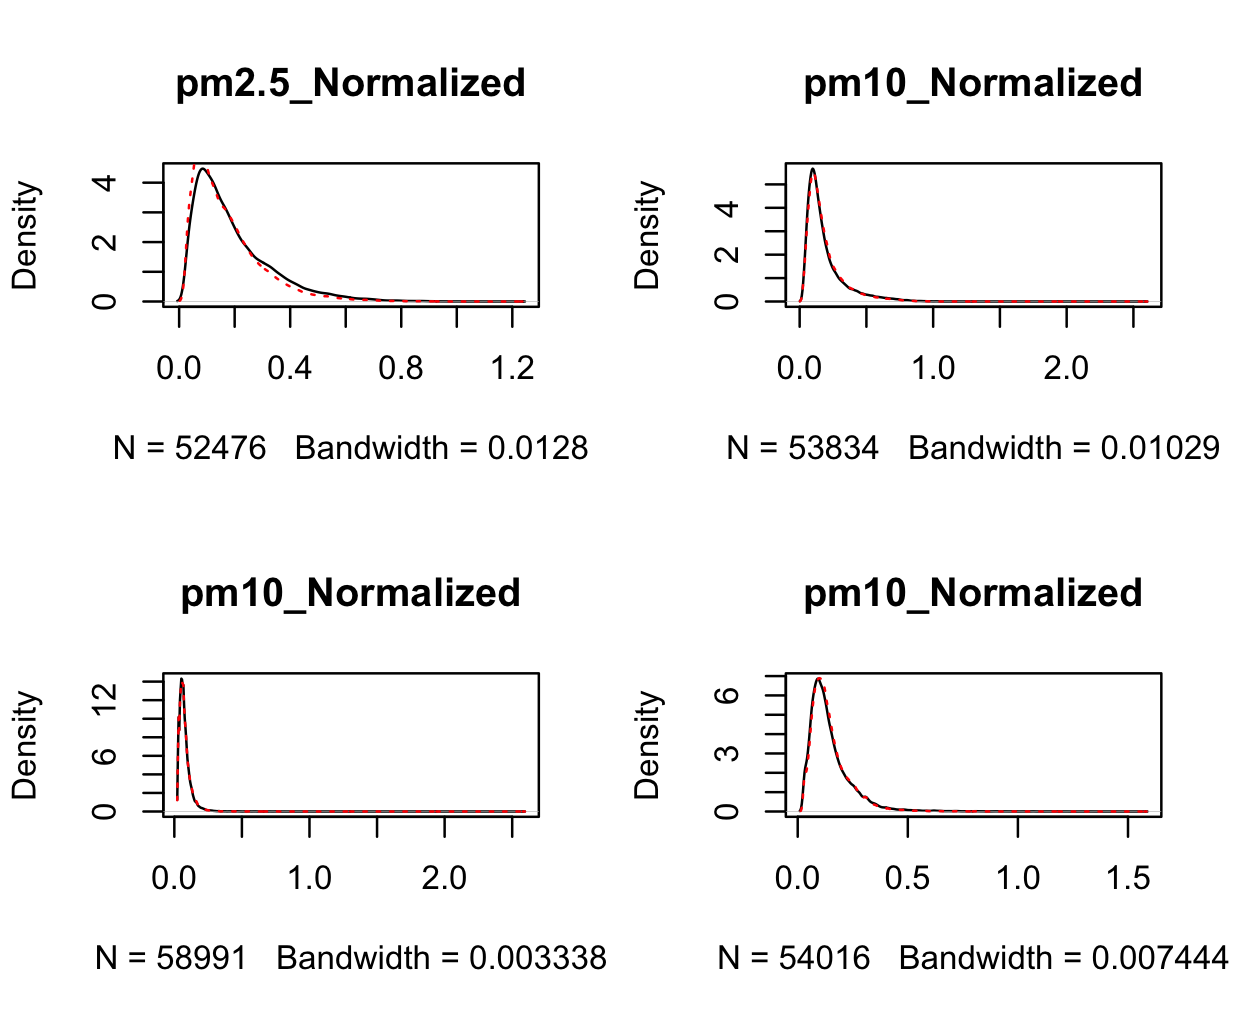
\includegraphics[width=3.125in,height=\textheight,keepaspectratio]{images/figure_2c.png}
\caption{Figure 2b. Data gap filling}
\end{figure}

(1)

\newpage

\subsection*{References}\label{references}
\addcontentsline{toc}{subsection}{References}

\phantomsection\label{refs}
\begin{CSLReferences}{0}{1}
\bibitem[\citeproctext]{ref-Munkh2017}
\CSLLeftMargin{1. }%
\CSLRightInline{\textbf{Munkhtsetseg E}, \textbf{Shinoda M},
\textbf{Ishizuka M}, \textbf{Mikami M}, \textbf{Kimura R},
\textbf{Nikolich G}. 2017. Anthropogenic dust emissions due to livestock
trampling in a mongolian temperate grassland. Atmospheric Chemistry and
Physics \textbf{17}:11389--11401.
doi:\href{https://doi.org/10.5194/acp-17-11389-2017}{10.5194/acp-17-11389-2017}.}

\end{CSLReferences}

\end{document}
